\chapter{Introduction}
\label{chapter:intro}

\paragraph{Summary}


\section{Cryptography}

Cryptography is the mathematical science of protecting secret information by transforming it into a form which is illegible. Generally, the original secret information is called the plaintext while the transformed information is called ciphertext. Once the plaintext is transformed into ciphertext, it can be sent over an insecure channel to its destination. At the destination, the reverse transformation takes place yielding back the original information. Transformation of plaintext to ciphertext is referred to as encryption, while the reverse process is called decryption.

% symmetric and asymmetric key cryptosystems

Symmetric key cryptosystems are classified into two types, based on the manner in which plaintext is used by the encryption algorithm. As mentioned earlier, these types are block ciphers and stream ciphers. Block ciphers divide the plaintext into blocks of data, and each such block is then encrypted. 

% explain block cipher

% explain stream cipher

An important point where stream cipher differs from block cipher is the usage of the key in encryption or decryption. While block ciphers use the secret key directly for encryption and decryption, in stream ciphers the secret key is used indirectly. The secret key is used to initialize a pseudo-random number generator, which is the most important component of the stream cipher design. 



\section{Stream cipher}

\subsection{One-time pads} 

Before we explain the working of stream ciphers, it is important that we understand the motivation for the design of stream ciphers. An inspiration behind practical stream ciphers of today has been the one-time pad, which is also known as the Vernam cipher. In the one-time pad, the length of the key is required to be equal to or greater than the length of the plaintext. Each plaintext bit is operated with the corresponding key bit using the \emph{exclusive-or} (or \emph{xor}) operation, thus resulting in one bit of the ciphertext. So, if $p_i$ represents the $i^{th}$ bit of the plaintext, and $k_i$ represents the $i^{th}$ bit of the key, then the $i^{th}$ bit of the ciphertext is given by $c_i$ = $p_i \oplus k_i$. The corresponding decryption takes place as $p_i$ = $c_i \oplus k_i$. This is shown in the figure ?.

The key bits are required to be completely random, without any statistical correlation between them. With this pre-condition, there is no way that an adversary could determine the secret key just by knowing the ciphertext. Since the key is derived from a truly random source, there could be several combinations of the plaintext and the key which result in the given ciphertext. The adversary would, in such a scenario, never be able to determine which of the specific combination is the right one, even with infinite computing power at hand.
% more on this
Shannon in 1975, used his notion of information theory to formally prove that one-time pads are unbreakable, and termed them as having perfect secrecy.

But for practical purposes, one-time pads have several weaknesses. These are explained in the following two points.
\begin{itemize}
\item The length of the key has to at least be equal to the length of the plaintext, if not greater than it, such that all the plaintext bits are encrypted. Thus, in order to encrypt large number of plaintext bits, large number of `random' key bits would have to be generated. Managing such a huge set of key bits is not practical, since the storage and transfer need to be carried out securely. 

\item In one-time pads, based on their name, a same key cannot be used for more than one computations. If the same key is used for encrypting two different plaintext messages, the chances that the key being broken are extremely high. The chances of the key being broken is precisely zero when the key is used just for one encryption round and is derived from a true random source. But, the same chances are extremely high if the key is reused. 
\end{itemize}

Considering the above points, rather than transmitting the key then, it is a better idea to transmit the plaintext itself through the secure channel, since the length of the key is equal to the plaintext and the key can just be used once. Clearly, one-time pads are not good enough for being deployed in practical systems, but they reveal a strong design basis for stream ciphers. The component missing between one-time pads and stream ciphers is the pseudo-random sequence generator, which is discussed next. 

% still, one-time pad is useful. explain. 

\subsection{Pseudo-random sequence generators}
\label{sec:psrg}

Pseudo-random sequence generator (PRSG) is used to derive a seemingly random sequence of bits called the \emph{keystream}, using a small initial seed value. PRSG's are finite state machines having an internal state, which is initialized using the secret key, along with some more initialization parameters if required. There are two important functions part of the PRSG. These are:
\begin{itemize}
\item A linear \emph{update function} is used to derive the next state using the current state.
\item A linear or non-linear \emph{output function} is used to generate an output bit from the current state. 
\end{itemize}

A stream of these output bits (occuring as the PRSG changes states) constitutes the keystream, which is used in stream ciphers. It is important to note that the keystream is not truly random, but as the name of the generator suggests, it is pseudo or seemingly random. 

%-----
% figure PRSG
%-----

\paragraph{Use in stream cipher construction:}
\label{para:stream-construction} 
Stream ciphers use secret keys of fixed length independent of the length of plaintext. Typically the key lengths are 128, 256 or 512 bits, which are considered secure by the computational power existing today. % check this and need a reference here %
The key is used to create the keystream, which replaces the long secret key in the one-time pads. The trade-off here is that the keystream is not truly random, since it is derived using the secret key and a pseudo-random bit generator. As a result, the perfect secrecy of one-time pads does not apply to stream ciphers, but at the same time, the strength of the pseudo-random sequence generator becomes extremely important in determining how strong the stream cipher is cryptographically.

An overview of a stream cipher design is shown in figure ?. The secret key is used to initialize the internal state of the pseudo-random sequence generator. Once the initial state is prepared, the pseudo-random sequence generator is ready to generate a stream of random looking bits or the keystream. Bits of the plaintext are consumed alongwith corresponding bits from the keystream to generate a stream of encrypted bits. In effect, the plaintext and the keystream are used to produce the ciphertext.

At the receiver end, the pseudo-random sequence generator is initialized using the shared secret key and the additional parameters which were used at the sender end. Any change in the initialization of the pseudo-random bit generator would result in a different keystream being produced, which would lead to incorrect decryption of the received ciphertext. Using the keystream, the ciphertext is decrypted to give the plaintext. 

% security of PRSG %
As briefly mentioned before, the security of the stream cipher much depends on the security properties of PRSG. The output sequence is required to behave as a true random sequence. The major considerations in achieving this requirement are mentioned below.
\begin{enumerate}
\item The period of the keystream should be large. This becomes extremely important when the length of the plaintext is large. If the keystream repeats, the same sequence would then be encrypting different parts of the plaintext. If the attacker has knowledge of some initial part of the plaintext, then the initial keystream encrypting that part can be recovered. This repeating keystream can further be used to decrypt part of the ciphertext which the attacker does not know. Even if no knowledge of plaintext is available to the attacker, certain properties about the plaintext can be derived from the two ciphertexts which are encrypted using the same keystream.

On the other hand, the requirement on how large the period should be depends on the particular application.
% reference robshaw
\item The 
\end{enumerate}

\subsection{Linear feedback shift registers} 
\label{sec:lfsr}
The most widespread implementation of PRSG's is done using a linear feedback shift register (LFSR). Other methods for generating pseudo-random sequences do exist as well. Since we are mainly going to deal with the use of LFSR based generators in this thesis, we would concentrate only on them. Other methods of generating pseudo-random sequences are linear congruence generators and non-linear feedback shift registers. It is important to note that LFSR provides only the \emph{update function} of the PRSG. The \emph{output function} of the PRSG needs to be implemented on top of the LFSR.
% reason why LFSR are widely used, and why are we more interested in them %
% more info on other generators %

A LFSR consists of two important components. These are explained below. 
\begin{enumerate}

\item \emph{Shift Register.} A shift register holds a fixed number of bits, and shifts each of them into corresponding adjacent positions (all towards a particular direction), upon the arrival of a clock cycle. If the direction of the shift is considered to be rightwards, then in every clock cycle, there is a new bit on the leftmost position of the register, and the rightmost bit is excluded from the register. Consider the figure ??.  If the $n$ bits of the shift register are represented by $s_0$, $s_1$, $s_2$ $\ldots$ $s_{n-1}$, then on every clock cycle, we have the following transformations: $s_{out}$ = $s_{n-1}$, $s_{n-1}$ = $s_{n-2}$ $\ldots$ $s_2$ = $s_1$, $s_1$ = $s_0$, $s_0$ = $s_{new}$; where $s_{out}$ is the bit which is excluded and $s_{new}$ is the new bit. What is done with the $s_{new}$ and $s_{out}$ bits depends on the application using the shift register. 

For example, one of the uses of shift registers has been in the conversion of sequential (or serial) data to parallel data, and vice versa. A sequence of bits can be stored in the shift register over a period of $n$ clock cycles, and retrieved in a parallel form in the $(n+1)'th$ clock cycle. In this case, $s_{new}$ bits are taken from the input sequential stream and $s_{out}$ bits are not used. For parallel-to-sequential data conversion, a parallel stream of bits could be fed into the shift register in one cycle, and retrieved sequentially over the next $n$ clock cycles. The bit $s_{new}$, in this case, may be set to a default value like \emph{0} (since it is not being used later) and $s_{out}$ would hold bits of the sequential output stream. 

%-----
% figure serial-to-parallel and parallel-to-serial conversion
%-----

\item \emph{Linear feedback.} A feedback function defines the $s_{new}$ bit as a function of the $n$ bits of the shift register. If the function is linear, it would be called \emph{linear feedback function}. Linearity is incorporated in the design by the use of $xor$ as the feedback function. Other boolean functions which are linear are negation, logical biconditional, tautology, and contradiction. According to [Wikipedia], 
\begin{quote}
A Boolean function is linear if A) In every row of the truth table in which the value of the function is 'T', there are an even number of 'T's assigned to the arguments of the function; and in every row in which the truth value of the function is 'F', there are an odd number of 'T's assigned to arguments; or B) In every row in which the truth value of the function is 'T', there are an odd number of 'T's assigned to the arguments and in every row in which the function is 'F' there is an even number of 'T's assigned to arguments.
\end{quote}

One way of designing feedback, as mentioned above, is to define $s_{new}$ as a function of the $n$ bits of the shift register. An LFSR based on such a function is called \emph{Fibonacci LFSR}. A different type of LFSR, called \emph{Galois LFSR}, implements the linear function between some specific bits of the shift register. Thus, the shift register no longer shifts bits directly to adjacent positions, but does apply a function on some of the bits before shifting them. Such an LFSR can be seen in figure ??. It is important to note here that we are going to concentrate only on Fibonacci LFSR's in this thesis. As a result, in the remaining part of this thesis, the use of LFSR would refer to a Fibonacci LFSR, unless otherwise quoted.

%-----
% figure Galois LFSR
%-----

\end{enumerate}

A simple example of an LFSR is shown in figure ??. Let us examine the linear feedback function more closely now. As we can see, certain selected bits from the shift register are xor'd, and the resulting bit is assigned to the leftmost bit in the next clock cycle. As a result, the internal state of the LFSR is changed. If we number the bits as \emph{1, 2,} $\ldots$ $, n$, then the bits 11, 13, 14 and 16 are used in the feedback function. These bits are referred to as \emph{tap sequence} or $taps$ of the LFSR. In general, the outputs that effect the input of the LFSR are called $taps$.

\paragraph{Maximal length tap sequence:} Based on this tap sequence, the complete cycle of various states of the LFSR is determined. Depending on the initial state, the LFSR would run through a set of states, and then return back to the initial state. This forms a cycle of states, which depends on the intial state chosen. In order to use the LFSR for generating a pseudo-random sequence, we want to have the longest cycle of the LFSR states. In other words, we want the LFSR to traverse through all possible states, which is equal to $2^n$, where $n$ is the number of bits in the shift register. This is important since it is desired that the pseudo-random sequence has a large period, as mentioned in the requirements for PSRG in section \ref{para:stream-construction}.

It should also be noted that, if the LFSR is in a state where all the bits are \textbf{0}, then the next state would also be the same. This condition occurs because the \textit{xor} of any number of \textbf{0}'s is always \textbf{0}. Such a state is called the \textit{trivial state}. As a result, no cycle is formed if this state is the initial state or an existing cycle is terminated if this state occurs in between the transitions. Hence the maximum number of different states in the LFSR becomes $2^n-1$. A tap sequence which generates a transition of states such that the period of the LFSR is $2^n-1$, is called the maximal length tap sequence. The first requirement the LFSR should satisfy is to contain a maximal length tap sequence, as this would guarantee that its period is the largest possible. The next step is to determine if a given tap sequence is a maximal length tap sequence or not. 

\paragraph{Polynomial representation of tap sequence:} Once we have a tap sequence, we can express it in the form of a polynomial with mod 2 coffecients. For the example shown in figure ??, the polynomial representation of the tap sequence is

\begin{center}
p(x) = $x^{16}$ + $x^{14}$ + $x^{13}$ + $x^{11}$ + 1
\end{center}

The powers of $x$ represent the tap bits. The \textbf{1} in the end, is a result of $x^0$ and represents the $s_{new}$ bit, since $s_{new}$ can be interpreted to be existing at the \textbf{0}'th position of the shift register. $s_{new}$ becomes $s_1$ in the next clock cycle, so in the current clock cycle, $s_{new}$ is $s_0$, which theoretically exists.

We now discuss the properties which the polynomial representation should satisfy, in order to  a maximal length LFSR. These are the properties of a \textit{primitive polynomial} in algebra. In other words, if the polynomial representing the LFSR is a primitive polynomial, then the the polynomial represents a maximal length LFSR. 

% properties of primitive polynomials %

\subsection{Some stream ciphers}

\section{The HiTag2 stream cipher}
\label{sec:hitag2}

\subsection{Background}

HiTag2 is a stream cipher originally designed by Philips Semiconductors (now NXP Semiconductors) and used for mutual authentication between a car remote control and controller in the car. Such systems (called remote keyless entry or RKE system) have been widely implemented in modern electronic cars, and facilitates unlocking of car doors upon just a button press from within a certain maximum distance from the car. The HiTag2 stream cipher provides two-way authentication, authenticating each of the two entities to each other one by one. But, this is just one use of the cipher, and other applications could use the cipher for authentication as well as encryption. It is important to understand here that if a stream cipher is used for authentication, the keystream bits are sent directly, since the challenge/response nonces are sent in plain previously. Hence, \emph{xor} of the nonce and keystream would hide nothing. While when encryption is desired, the message bits are \emph{xor}'d with the keystream bits before sending over the public channel. 

HiTag2 was kept secret by Philips until it was reverse-engineered using the cipher's software implementation. The microcode (or assembly code) of HiTag2 was decompiled from the implementation available in the car remote controls and the RKE receivers. The C code for the cipher is availabe on the website \cite{hitag2-code}. A full system level specification of the RKE system by Philips (titled Active Tag and IC) implementing the HiTag2 cipher is available \cite{active-tag-datasheet}. HiTag2 now is the intellectual property of NXP, but the specification document holds the name of Philips since NXP did not come into existence at that time in 2005. Also, since the cryptography (HiTag2) on the RKE system was kept secret at that time, HiTag2 modes are just mentioned without any further information on the functional working of the cipher.

The design of HiTag2 is very similar to a recently reverse-engineered \cite{NohlESP-2008-usenix} stream cipher called Crypto-1, which is used in Mifare Classic smartcards by NXP. The Mifare family comprises of contactless smart cards and card readers, with a variety of different features including memory availability on the cards to store data and read/write permissions on the cards. As a result of these features, Mifare system is widely used in applications requiring more than just authentication. Some such applications are ticketing system for public transportation (OV-Chipkaart in Netherlands, Oyster cards in UK etc.) and access control in buildings. Crypto-1 cipher used in Mifare Classic cards and readers was proprietary until recently when Nohl et. al. \cite{NohlESP-2008-usenix} reverse-engineered the algorithm from its silicon implementation.

In addition, the same Mifare Classic cards and readers are shown to be easily clonable \cite{dekoninggans2008pam} by researchers at Radboud University. They have analyzed the communication protocol between Mifare Classic cards and readers, and have been been able to show that the there are several weaknesses in the Crypto-1 cipher. They have been able to recover the necessary keystream by analyzing the protocol messages. The details of this protocol analysis complements the work by Nohl et. al., and using both the ideas, mounting brute-force attacks on the cipher have been made possible. 

Apart from reverse-engineering from software or hardware implementations, a black-box reverse-engineering has also been applied to break secret algorithms. The DST RFID tag (using the DST stream cipher) was broken in 2005 using black-box reverse-engineering \cite{bono2005sac}, i.e. by selecting certain input formats and using both the input and output combinations to deduce the structure and working of the cipher. The most common application of Texas Instrument's DST tag is in vehical immobilizer systems and electronic payment systems \cite{dst-rfid-analysis}. 

Next, we describe the working of the HiTag2 cipher, and after that we carry out a brief security analysis of the cipher.

\subsection{Cipher Description}
The various components of the HiTag2 stream cipher are outlined below. 
\begin{itemize}
\item 48 bit key
\item 32 bit serial ID
\item 32 bit initialization vector (IV)
\item 48 bit internal state with linear update function (basically, an LFSR)
\item Non-linear output function based on multiplexor, with fixed data bits and address bits depending on the current internal state
\end{itemize}

The entire setup of the keystream generator is done in two phases. The first phase is the initialization of the LFSR, which sets the internal state to a non-zero value using the key and the serial ID. The second phase is the setup of the LFSR during which the LFSR is clocked (resulting in the shifting of bits) and the key and IV bits are used in the process. Once the LFSR is set, the keystream is ready to be generated from the internal state right away. We describe these phases in detail here.\\ 

\textit{\textbf{1. LFSR Initialization.}} The initialization step of the LFSR is straightforward. Instead of initializing the LFSR with zeros, the bits are initialized with the serial ID and initial part of the key. The 32 bits of the serial ID (from \emph{lsb} to \emph{msb}) are stored in the first 32 bits of the LFSR (bits from index 0 through index 31). Then, the first 16 bits of the key (again, from \emph{lsb} to \emph{msb}) are stored in the remaining 16 bits of the LFSR (bits from index 32 through index 47). With this the initialization of the LFSR is complete. This is also shown in figure \ref{fig:hitag2-1}.\\

\begin{figure}[ht!]
	\centering
		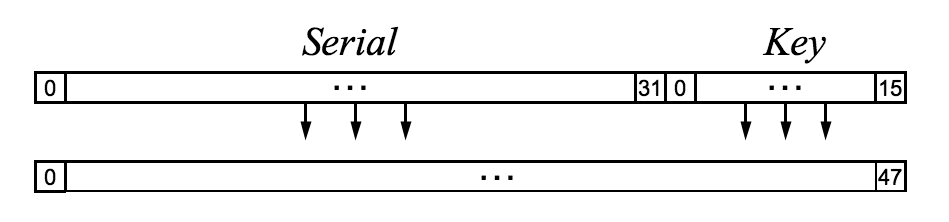
\includegraphics[width=5in]{./figures/hitag2-1.PNG}
	\caption{LFSR Initialization}	
	\label{fig:hitag2-1}
\end{figure}

\textit{\textbf{2. LFSR Setup.}} During the setup of the LFSR, the 32 bits of IV are used with the remaining 32 bits of the key. The bits in the LFSR are shifted to the right in every clock cycle, and a new value is stored in the leftmost bit (refer section \ref{sec:lfsr}). In every clock cycle, an xor of three bits: one bit from the remaining part of the key (bits from index 16 through 47), one bit from the IV (from \emph{lsb} to \emph{msb}) and the output bit from the non-linear output function, is stored at the leftmost bit of the LFSR. After 32 clock cycles, the internal state is now prepared for keystream generation. This is shown in figure \ref{fig:hitag2-2}.\\

\begin{figure}[ht!]
	\centering
		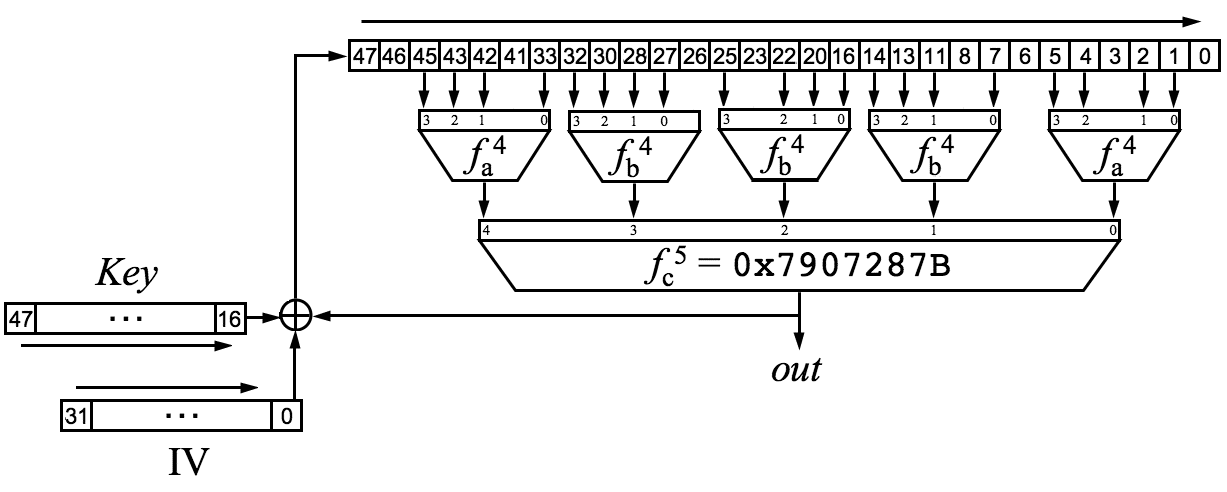
\includegraphics[width=5in]{./figures/hitag2-2.PNG}
	\caption{LFSR Setup Phase}	
	\label{fig:hitag2-2}
\end{figure}

\textit{\textbf{Output function.}} The output function consists of two levels of sequentially arranged multiplexors. The multiplexors have pre-decided data bits, where as the address bits are chosen either from the LFSR or from other multiplexors. In the first level, 20 bits from the LFSR are used as address bits to five four-bit multiplexors, giving a total of five bits of output (one from each multiplexor). These five bits are then used as address bits to the single five-bit multiplexor at the second level. The output bit of this multiplexor gives the stream cipher's keystream bit. In all, six instances of multiplexors cover the two levels of the output function.

Three different multiplexor functions are used to realize these six instances, and these are called $f_a^4$, $f_b^4$ and $f_c^5$. While $f_a^4$ and $f_b^4$ take in four bits for addressing the output, $f_c^5$ takes in five bits. The multiplexors $f_a^4$ and $f_b^4$ are used in the first level, where as $f_c^5$ is used in the second level. The six different instances of these functions used are described in the table \ref{tab:muxs}. In the table, the input bits for the first level of multiplexors are indicated by indices of LFSR bits.

\begin{table}[ht!]
\begin{center}
\small{
\begin{tabular}{|p{2.2cm}|l|p{2cm}|p{2.8cm}|p{1.5cm}|}
\hline
\textbf{Multiplexor instance}	& \textbf{Function}		& \textbf{Data bits}	& \textbf{Address bits (input)}		& \textbf{Output bit}\\ \hline
\multicolumn{5}{|c|}{Level 1 Multiplexors}\\ \hline
MUX 1 			&	$f_a^4$			& 0x2C79			& 1, 2, 4, 5							& $o_1$\\
MUX 2 			&	$f_b^4$			& 0x6671			& 7, 11, 13, 14						& $o_2$\\
MUX 3 			&	$f_b^4$			& 0x6671			& 16, 20, 22, 25					& $o_3$\\
MUX 4 			&	$f_b^4$			& 0x6671			& 27, 28, 30, 32					& $o_4$\\
MUX 5 			&	$f_a^4$			& 0x2C79			& 33, 42, 43, 45					& $o_5$\\ \hline
\multicolumn{5}{|c|}{Level 2 Multiplexor}\\ \hline
MUX 6 			&	$f_c^5$			& 0x7907287B	& $o_1$, $o_2$, $o_3$, $o_4$, $o_5$		& $k_i$\\ \hline
\end{tabular}}
\end{center}
\caption{Multiplexors making the output function}
\label{tab:muxs}
\end{table}

Hence, as mentioned previously, the output bit from the function $f_c^5$ is \emph{xor}'ed with the key and IV bits for 32 clock cycles and written to the rightmost bit of the LFSR.

The source code for the initialization and setup of the LFSR is shown below in the listing. Here, the function \emph{f20()} stands for the output function, which we have just described.\\

\lstinputlisting[frame=trBL, caption={HiTag2 initialization code snippet}]{./code-snippets/hitag2_init.c}

\textit{\textbf{3. Keystream Generation.}} The output from the function $f_c^5$ constitutes the keystream. In addition, the LFSR state is changed in every clock cycle through the update function. The internal state is updated linearly, in the following fashion: an xor of the taps of the LFSR (which are bits 0, 2, 3, 6, 7, 8, 16, 22, 23, 26, 30, 41, 42, 43, 46 and 47) is written to the leftmost bit of the LFSR. Once the internal state is changed, the output bit gets recomputed, generating the next bit of the keystream. This is shown in figure \ref{fig:hitag2-3}. Following is the code snippet for the function implementing one round of the HiTag2 (\emph{hitag2\_round}), by first updating the state and then calling the output function (\emph{f20}).\\

\lstinputlisting[frame=trBL, caption={HiTag2 keystream generation code snippet}]{./code-snippets/hitag2_round.c}

\begin{figure}[ht!]
	\centering
		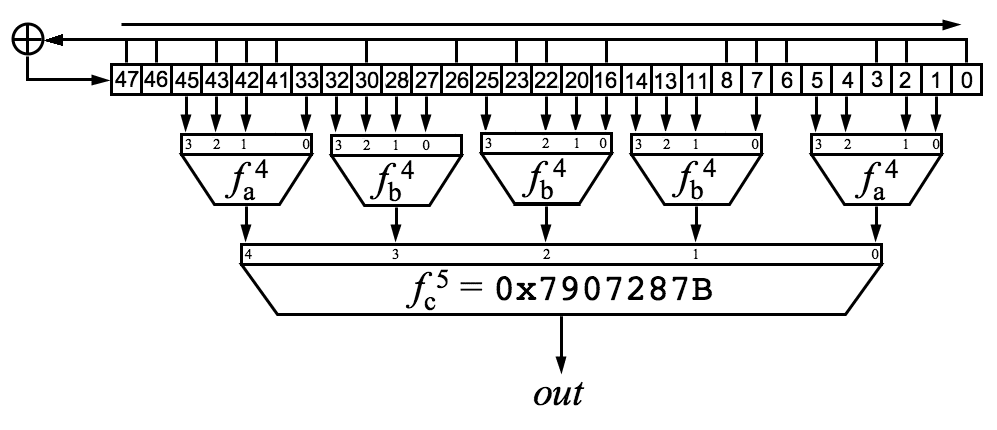
\includegraphics[width=5in]{./figures/hitag2-3.PNG}
	\caption{Keystream Generation}	
	\label{fig:hitag2-3}
\end{figure}

\subsection{Brief security analysis}
% a basic cryptanalysis of the cipher - maximal period? linearity? %
